\documentclass[/home/greg/Thesis/main/main.tex]{subfiles}

\begin{document}
\graphicspath{{/home/greg/Neutron_star_modelling/MotionOfARigidBody}}
\newcommand{\MotionOfARigidBodyDir}{/home/greg/Neutron_star_modelling/MotionOfARigidBody}

\FloatBarrier
As \citet{Landau1969} described, the motion of $\mathbf{M}$ in the rotating frame
can be understood from by conservation laws. For the time being let us consider,
in the rotating frame, a torque free body with moments of inertia $I_{1}, I_{2}, I_{3}$. 
If the spin-vector components are given by $M_{i} = I_{i} \Omega_{i}$ then 
in momentum space, we can write the conservation of energy and angular momentum as
\begin{align}
    \frac{M_{1}^{2}}{I_{1}} + \frac{M_{2}^{2}}{I_{2}} + \frac{M_{3}^{2}}{I_{3}} = 2E 
    \label{eqn: ellipse} \\
    M_{1}^{2} + M_{2}^{2} + M_{3}^{2} = M^{2}
    \label{eqn: sphere}
\end{align}
The conservation of energy describes an ellipsoid with semi-axis
$\sqrt{2EI_{1}}, \sqrt{2EI_{2}}$ and $\sqrt{2EI_{3}}$. The conservation of 
angular momentum describes a sphere of radius $M$. The intersection of the
sphere and ellipse at fixed $E$ and $M$ describe the precession of the angular
momentum and hence the spin-vector.

\section{Torque free biaxial body}
For a biaxial body free from torques we can parameterise the principle components
of the moment of inertia by 
\begin{align}
    I_{1} = I_{2} = I_{0}, &&& I_{3} = I_{0}(1 + \epsI)
\end{align}
For such a system, the Euler rigid body equations have an
exact solution with $\Omega_{3}=$ const and the other components are given by
\begin{align}
    \Omega_{1} = \left(\Omega^{2} - \Omega_{3}^{2}\right)^{1/2}\cos\left(\epsI \Omega_{3} t\right),\\
    \Omega_{2} = \left(\Omega^{2} - \Omega_{3}^{2}\right)^{1/2}\sin\left(\epsI \Omega_{3} t\right),
\end{align}
where $\Omega^{2}$ is also a constant since there is no torque. In the rotating
body frame this solution demonstrates that the spin-vector will precess in a
circle about the symmetry axis. The circle is precisely the intersection of the
ellipsoid and sphere. Since the cone is aligned with the $3$ axis, we can define
a polar angle $\theta$ made by the spin-vector with the $3$ axis. This will be 
constant during a precessional period and can be calculated as follows:
\begin{equation}
\sin\theta = \frac{M_{3}}{M}
\label{eqn: sin theta}
\end{equation}

\begin{figure}[htb]
\centering
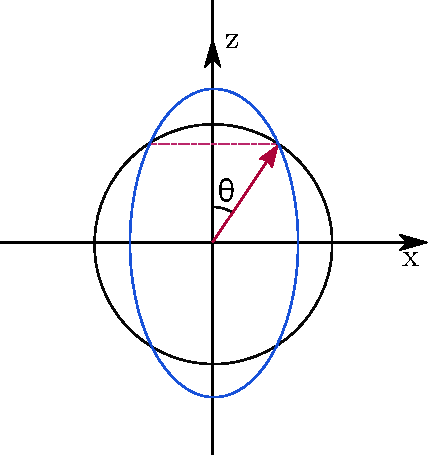
\includegraphics[width=0.4\textwidth]{\MotionOfARigidBodyDir/../Illustrations/SphereEllipse/SphereEllipseBiaxial}
\caption{}
\label{}
\end{figure}

From equation \eqref{eqn: ellipse} we can rearrange
\begin{align}
    M_{3}^{2} & = (1+\epsI)\left(2EI_{0} - M_{1}^{2} - M_{2}^{2}\right) \\
              & = I_{0} (1+\epsI)\left(2E - I_{0}\left(\Omega^{2} - \Omega_{3}^{2}\right)\right)
\end{align}
and similarly
\begin{align}
    M^{2} & = M_{1}^{2} + M_{2}^{2} + M_{3}^{2} \\
          & = I_{0}^{2}\left(\Omega_{1}^{2} + \Omega_{2}^{2}\right) 
    + I_{0}(1 + \epsI)\left(2E - I_{0}\left(\Omega^{2} - \Omega_{3}^{2}\right)\right)\\
          & = I_{0}^{2}\left(\Omega^{2} - \Omega^{3}\right)
    + I_{0}(1 + \epsI)\left(2E - I_{0}\left(\Omega^{2} - \Omega_{3}^{2}\right)\right)\\
    & = I_{0}\left(2E + \epsI \left(2E - I_{0}\left(\Omega^{2} - \Omega^{2}_{3}\right)\right)\right)
\end{align}
Then we can write the polar angle as
\begin{equation}
    \sin\theta = \left(\frac{(1+\epsI)\left(2E - I_{0}\left(\Omega^{2} - \Omega_{3}^{2}\right)\right)}
        {2E + \epsI\left(2E - I_{0}(\Omega^{2} - \Omega_{3}^{2})\right)}
    \right)
\end{equation}

\biblio
\end{document}

